\documentclass[11pt]{article}
\usepackage[margin=1in]{geometry}
\usepackage{graphicx}
\usepackage{booktabs}
\usepackage{amsmath}
\usepackage{multirow}
\usepackage{array}
\usepackage{caption}
\captionsetup{font=small,labelfont=bf}
\usepackage[colorlinks=true,linkcolor=black,citecolor=black,urlcolor=blue]{hyperref}

\newcommand{\pref}{\mathrm{pref}}

\title{The template channel dominates, the MSA selects, and sequence barely
matters: family-consensus conformational-state selection in an
AlphaFold3-style protein structure network}

\author{Cheng Ding$^{1,\ast}$\\
\small $^{1}$School of Life Science and Technology, ShanghaiTech University, Shanghai, China\\
\small $^{\ast}$Correspondence: \texttt{dingcheng2024@shanghaitech.edu.cn}}
\date{}

\begin{document}
\maketitle

\begin{abstract}
\noindent
Structure predictors of the AlphaFold family receive three conceptually
distinct inputs --- the query sequence, a multiple sequence alignment (MSA),
and structural templates --- and a substantial body of work on AlphaFold2
(AF2) has established a functional hierarchy among them: a strong MSA
overrides templates, and both dominate the bare sequence. Whether this
hierarchy survives the architectural redesign of AlphaFold3-style (AF3-style)
trunks --- in which the MSA is demoted to a single small module that writes
once into the pair representation, and the template track is trained directly
against noised ground-truth structures --- is unknown. We address this
question in RosettaFold-3 (RF3), an open AF3-style model, using a
distogram-based conformational-state preference score that asks, for 13
proteins with two experimentally resolved states, which state the network
favours under each input condition. Three results emerge. First, the MSA
acts as a \emph{family-consensus state selector}, not a generic
crystallographic-bias agent: it shifts RF3 away from the crystallized state
in KaiB and RfaH (shifts $-2.29$ and $-2.99$ in NLL units), toward it in
XCL1 and Mad2 ($+2.87$, $+0.91$), sharpens the sequence-intrinsic fold
preference of the designed GA88/GB88 pair ($+2.56$), and leaves a GPCR, two
kinases, a transporter and three X-ray-versus-NMR control pairs inside the
measured noise band. Second, the hierarchy of the input channels is
\emph{inverted} relative to AF2: experimental templates steer state
preference by $\pm 4$--$5$ units and override the MSA in direct conflict
on all tested targets (template $\pm 4$--$5$ $>$ MSA $\pm 2.7$ $>$
sequence $\pm 0.3$ on GA88/GB88), while on a deep mutational scanning
benchmark a wild-type crystal template is actively \emph{harmful}
($-0.049$ Spearman relative to no-MSA) where the MSA is helpful --- the
MSA is not a de facto template. Third, in a homodimer the MSA preferentially
amplifies the inter-chain block of the pair representation, but an unpaired
control shows this is amplification of a network-internal interface prior by
family context, not inter-chain coevolution. All conclusions are
model-specific to the AF3-style template channel and should not be
extrapolated to AF2-class architectures without retesting.
\end{abstract}

\section{Introduction}

A non-trivial minority of proteins adopt more than one stable, experimentally
characterizable conformation: metamorphic fold-switchers such as KaiB, RfaH,
Mad2 and lymphotactin (XCL1) refold secondary structure wholesale
\cite{porter2018,chang2015,burmann2012,luo2004,tuinstra2008}, while GPCRs,
kinases and transporters populate alternative functional states that differ
more modestly but consequentially. Deep-learning structure predictors,
trained on the Protein Data Bank and evaluated largely on single-state
accuracy, compress this plurality into one answer: AlphaFold2 (AF2) captures
only one of the two known conformers for the large majority of fold
switchers \cite{chakravarty2022,chakravarty2024}, and the AF3 authors
themselves note that their model ``typically predict[s] static structures as
seen in the PDB'' \cite{abramson2024}. Understanding \emph{which input
channel} decides the predicted state is therefore both a mechanistic question
about these networks and a practical one for anyone trying to sample
alternative conformations.

For AF2 the answer is well documented. The Evoformer couples a processed MSA
to the pair representation over many blocks \cite{jumper2021}, templates
enter as a separate and comparatively weak track, and when the two conflict,
the MSA wins: ``if the MSA signal is strong, AlphaFold tends to ignore
structural information from the template'' \cite{kovalevskiy2024}. An entire
methodological family exploits this hierarchy --- subsampling, clustering,
mutating or masking the MSA releases alternative conformational states
\cite{delalamo2022,stein2022,wayment2024,kalakoti2025} --- and removing the
MSA removes learned state biases in GPCR modelling \cite{heo2022,sala2023}.
The accepted ordering is thus MSA $>$ template $>$ sequence for
conformational control in AF2-class models.

The MSA itself entered structure prediction as the carrier of evolutionary
covariation: residue pairs that co-vary across a family tend to be in
contact, and coevolution-only methods could fold small proteins without any
structural training data \cite{marks2012}. AlphaFold1 distilled these
statistics into learned distance potentials \cite{senior2020}; AF2 made the
MSA a first-class, actively processed input. The field has since moved in
both directions at once. Single-sequence language models removed the MSA
while retaining most of its structure signal \cite{lin2023,hayes2024}, and
generative design models carry the structural prior entirely in pretrained
weights \cite{watson2023}. Yet both AF2 and AF3 retain a measurable
dependence on MSA depth \cite{jumper2021,abramson2024}, and alignment-based
statistics remain among the strongest substrates for variant-effect
prediction across MSA depths \cite{notin2023,akiyama2025}. The MSA is
neither dispensable nor neutral: it is a channel with real information
content whose conformational side effects are the subject of this paper.

AF3-style trunks reorganize these channels in ways that make the AF2 answer
non-obvious. The MSA is ``substantially de-emphasized'': four small blocks
integrate it by pair-weighted averaging, after which the MSA representation
is discarded and all information flows through the pair representation
\cite{abramson2024}. RosettaFold-3 (RF3), the open implementation we study,
follows this design \cite{corley2025}. In parallel, the template input was
upgraded to an atom-level track trained against noised ground-truth
structures \cite{corley2025} --- a training regime that could plausibly teach
near-literal copying, in contrast to AF2's heavily regularized template
path. Two channels with opposite directions of architectural travel
(demoted MSA, empowered template) motivate a direct re-measurement of the
hierarchy, and of what the MSA's conformational influence actually consists
in.

Existing evidence about MSA effects is almost entirely input-to-output:
perturb the MSA, observe structures or fitness correlations
\cite{delalamo2022,stein2022,wayment2024,saldano2022}. Two gaps matter here.
First, no study has quantified, inside an AF3-style trunk, how the MSA and a
template each move the network's conformational preference on proteins with
two known states. Second, the natural suspicion --- that an MSA acts as a
distributed, evolution-averaged template and that ``MSA bias'' is just
crystallographic bias in disguise \cite{heo2022,sala2023,kovalevskiy2024}
--- has never been tested by pitting a real template against a real MSA in
the same network, at the level of output state preference, internal
representation geometry, and downstream function.

We fill both gaps in RF3. On 13 two-state targets scored by distogram
negative log-likelihood (NLL) against both experimental reference
structures, we show that the MSA selects a family-consensus state with
target-dependent direction, that a ground-truth-trained template channel
dominates the MSA in direct conflict (inverting the AF2 hierarchy), that
template and MSA writes are qualitatively different objects (the template is
a stronger, mutation-erasing rewrite that harms variant-effect prediction,
the MSA a milder, family-consensus write that helps), and that the MSA's
amplification of inter-chain geometry in a homodimer reflects an internal
interface prior rather than paired-alignment coevolution. Throughout, we
report only quantities computed on shared residue universes after correcting
two analysis bugs (a span-mismatch/compression bug and a silently dropped
template input), and we flag single-forward noise limits explicitly.

\section{Results}

\subsection{A family-consensus state selector, not a crystal-bias agent}

We assembled 13 proteins with two experimentally resolved states each,
spanning fold-switchers (KaiB, RfaH, Mad2, XCL1, selecase, the designed
GA88/GB88 pair), a GPCR ($\beta$2AR), two kinases (Abl1, EGFR), a
transporter (LacY), and three same-construct X-ray-versus-NMR pairs
(ubiquitin, GB1, thioredoxin) that serve as near-null controls
(Table~\ref{tab:targets}). For each target we ran RF3 with and without its
MSA and scored the predicted distogram against both experimental C$\alpha$
distance maps on a shared residue universe, defining
$\pref = \mathrm{NLL}_B - \mathrm{NLL}_A$ (positive favours state A) and the
MSA-induced shift $\Delta\pref = \pref_{\mathrm{msa}} - \pref_{\mathrm{nomsa}}$.
Repeat forwards of identical inputs place the run-to-run noise band of
$\Delta\pref$ at roughly $\pm 0.14$--$0.27$; we treat shifts inside this
band as null (Methods).

\begin{figure}[t]
\centering
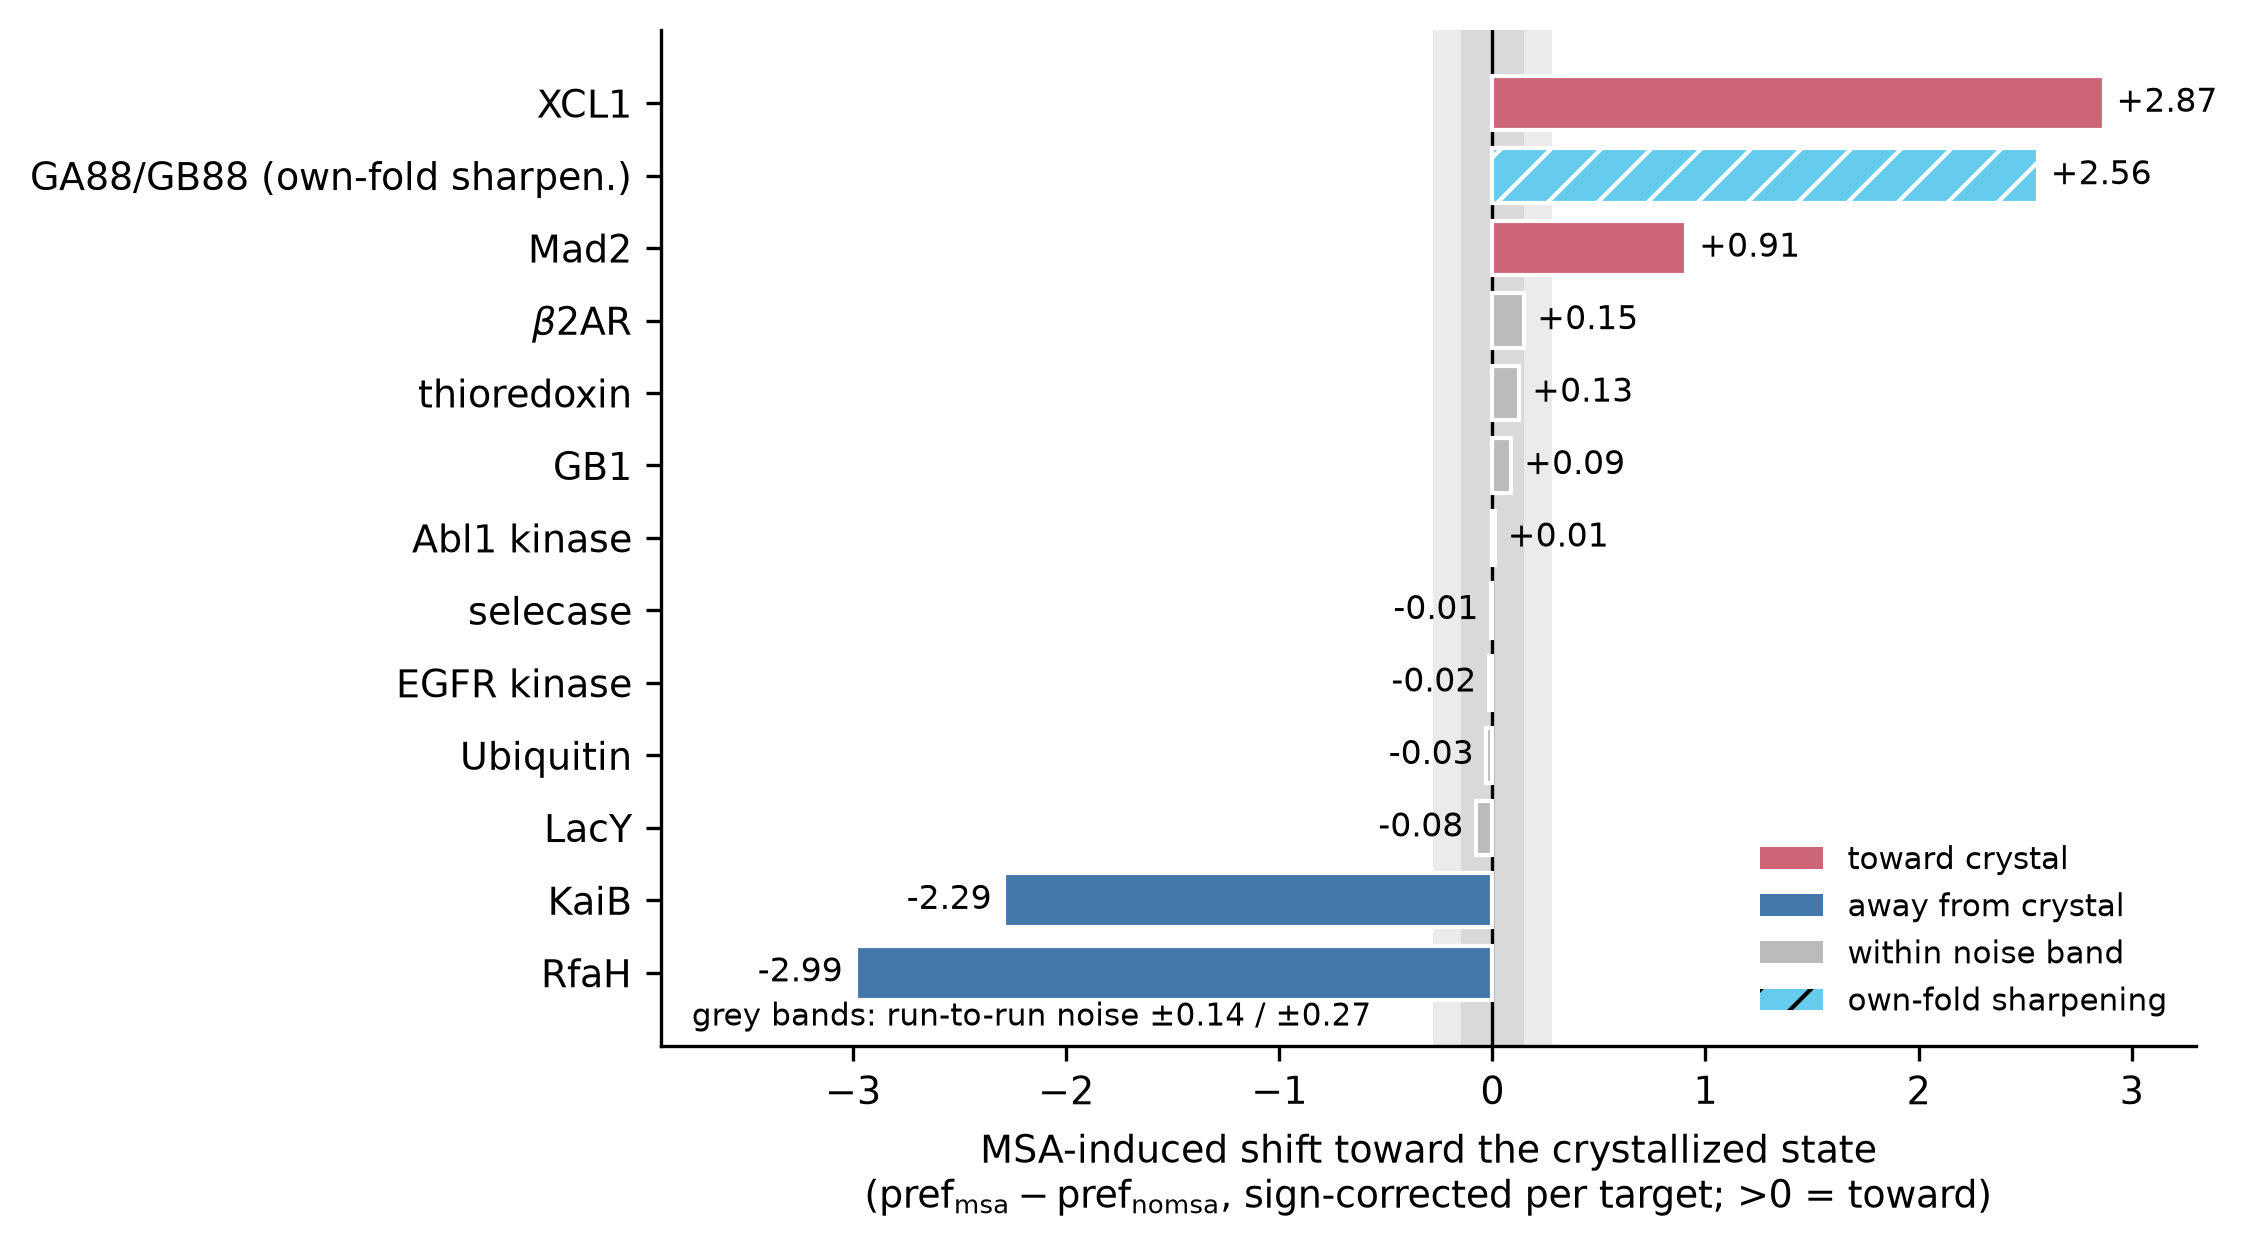
\includegraphics[width=0.98\linewidth]{figures/fig1_e2_shifts.png}
\caption{\textbf{The MSA shifts conformational state in a target-dependent
direction.} MSA-induced shift of the distogram state preference, sign
corrected so that positive values point toward the state that dominates the
PDB for that target (for Mad2 the crystallized state is state~B; the
GA88/GB88 entry is an own-fold sharpening score and has no crystallographic
direction). Shaded bands: run-to-run preference noise ($\pm 0.14$ inner,
$\pm 0.27$ outer). Red: significant toward-crystal; blue: significant
away-from-crystal; grey: within noise. All values from the range-matched
rescoring (Table~\ref{tab:targets}).}
\label{fig:e2}
\end{figure}

The result is not a uniform pull toward crystallized states
(Fig.~\ref{fig:e2}). Two fold-switchers are shifted \emph{away} from the
crystallized ground state toward the alternative, NMR-characterized fold:
KaiB ($\Delta\pref = -2.29$; the MSA reverses the sign of the preference,
$+0.72 \rightarrow -1.57$) and RfaH ($-2.99$; $+0.10 \rightarrow -2.89$).
Two others are shifted \emph{toward} the crystallized state: XCL1
($+2.87$; $-0.78 \rightarrow +2.09$) and Mad2 ($-0.91$ with state~B
crystallized; $-0.05 \rightarrow -0.96$). The designed 88\%-identical pair
GA88/GB88 shows a third behaviour: RF3 already predicts each sequence into
its own fold from sequence alone (GA88 $+0.38$; GB88 $-0.23$), and the MSA
\emph{sharpens} this intrinsic preference roughly tenfold
($+2.74$ and $-2.66$ respectively; $+2.56$ when GA88 is scored in the main
range-matched flow) rather than redirecting it. Finally, the membrane and
control targets sit at or inside the noise band: $\beta$2AR $+0.15$,
thioredoxin $+0.13$, GB1 $+0.09$, Abl1 $+0.01$, selecase $-0.01$, EGFR
$-0.02$, ubiquitin $-0.03$, LacY $-0.08$. We note explicitly that LacY and
EGFR, which appeared to shift toward the crystallized state in a preliminary
analysis ($+0.94$, $+0.31$), collapse to null once both states are scored on
a shared residue universe; the ``transporter/kinase/GPCR pulled toward the
PDB state'' pattern does not survive range matching, and we do not claim it.

The organizing principle that fits all four classes is that the MSA writes a
\emph{family-consensus} state. Where the family consensus coincides with the
crystallized state (XCL1, Mad2), the shift is toward crystal; where the
consensus favours the alternative fold (the KaiB and RfaH families, in which
the fold-switched form is the more common family member
\cite{chang2015,burmann2012}), the shift is away from crystal. Crystal bias
is thus a special case of consensus selection, not its definition --- echoing
output-level analyses of AF2 that attributed conformational pinning to
evolutionary consensus averaging rather than to the PDB distribution per se
\cite{saldano2022}. For near-identical designed pairs, the family level is
nearly uninformative and the MSA instead amplifies the sequence-encoded
preference, consistent with the observation that MSA subsampling fails to
release alternative states for some targets in AF2 as well \cite{stein2022}.

Two technical points deserve emphasis. First, the tally is: 2 targets
significantly toward crystal (XCL1, Mad2), 2 significantly away (KaiB,
RfaH), 1 sharpening (GA88/GB88), and 8 null --- so on a simple count the
MSA is \emph{inert} on the majority of our panel, and the secure signal
lives entirely in the fold-switching targets. Second, the controls behave
as controls should: the three X-ray-versus-NMR same-construct pairs and the
single-homolog selecase MSA give $|$shift$| \le 0.13$, so the distogram
readout does not manufacture crystal preference where the two reference
states differ only by experimental method, and a content-free MSA produces
no shift.

\subsection{The hierarchy inverts: template $>$ MSA $>$ sequence}

For the five targets with usable structures of \emph{both} states (KaiB,
RfaH, Mad2, XCL1, LacY), we additionally supplied each state structure as a
token-level template, alone (tplA, tplB) and in direct conflict with the MSA
(msa\_tplA: the MSA, whose direction was measured above, plus the template
of the state the MSA pushes \emph{away} from on KaiB/RfaH; the construction
is analogous on all five).

\begin{figure}[t]
\centering
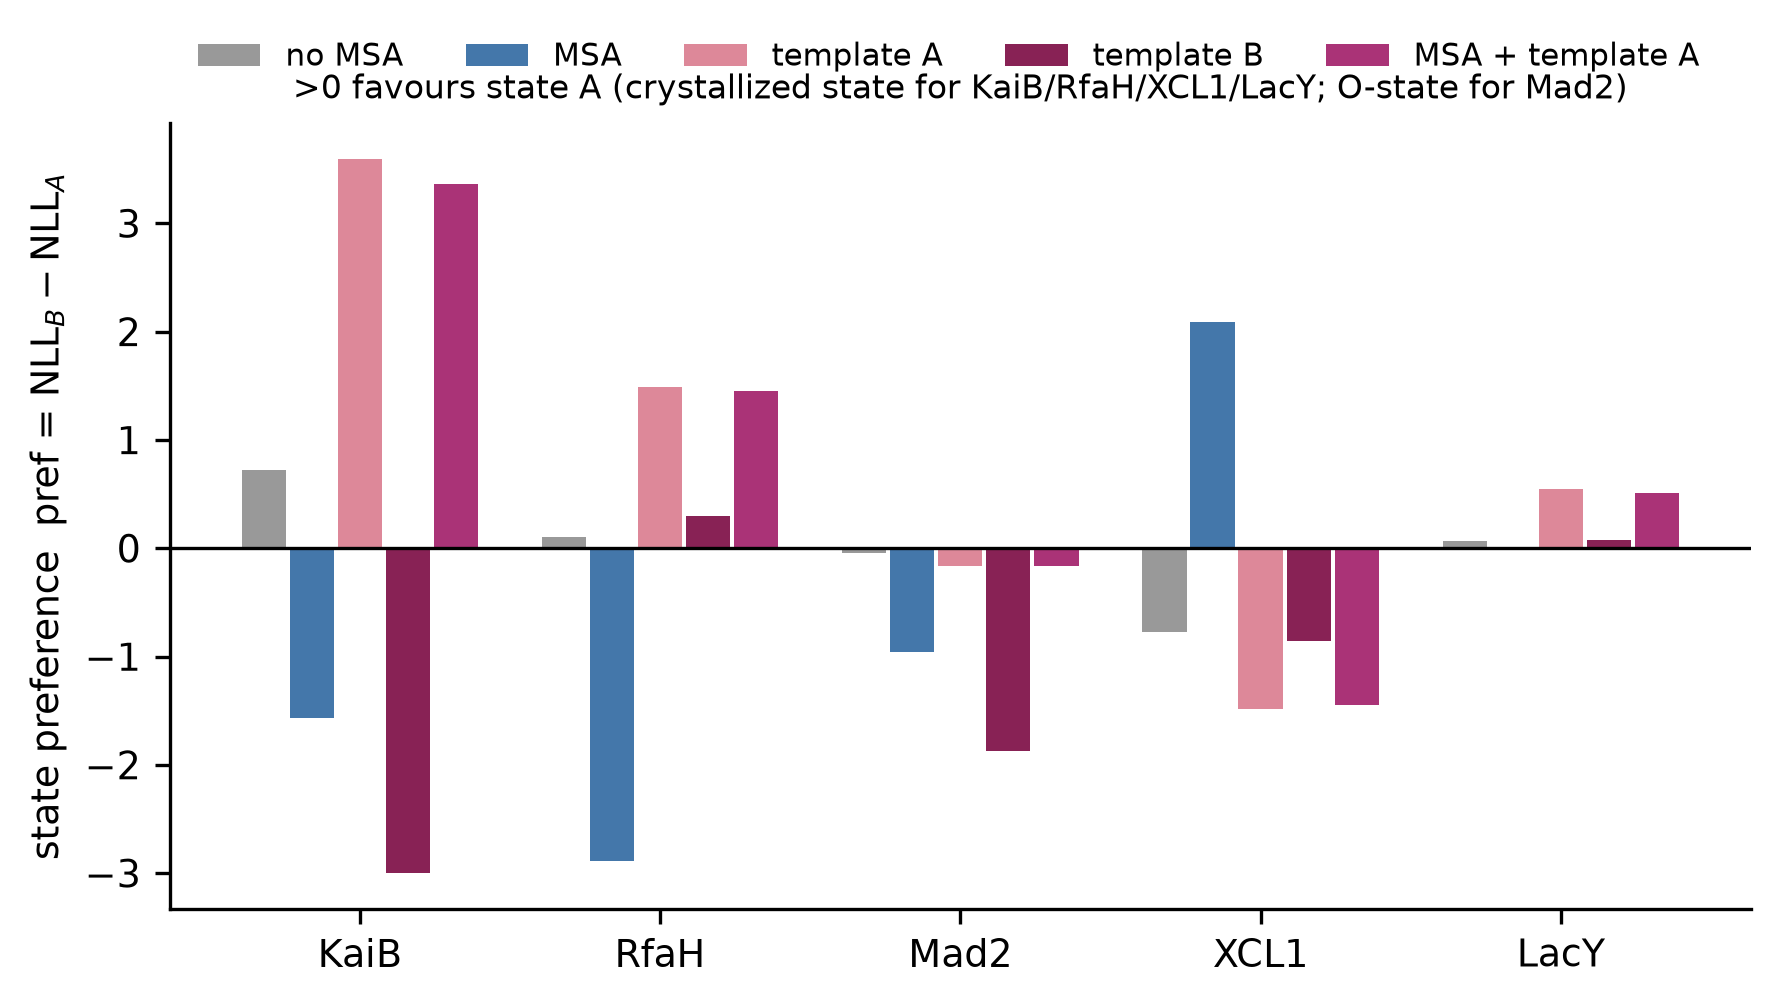
\includegraphics[width=0.98\linewidth]{figures/fig2_e49_arms.png}
\caption{\textbf{Templates steer strongly and bidirectionally; the MSA never
overrides a conflicting template.} State preference ($\pref =
\mathrm{NLL}_B - \mathrm{NLL}_A$; positive favours state A) for five
two-state targets under sequence-only, MSA, template-of-state-A,
template-of-state-B, and MSA-plus-template-A conditions. All values are
range-matched. Note the Mad2 anomaly: the O-state template (1DUJ, NMR) fails
to pull toward state A, while the C-state template works; see text.}
\label{fig:e49}
\end{figure}

Three observations stand out (Fig.~\ref{fig:e49}, Table~\ref{tab:e49}).
First, templates steer strongly and bidirectionally: the template-steering
span $\pref_{\mathrm{tplB}} - \pref_{\mathrm{tplA}}$ reaches $-6.59$ on KaiB
(tplA $+3.59$ vs tplB $-3.00$) and is directionally template-following on
all five targets (RfaH $-1.19$, Mad2 $-1.70$, LacY $-0.47$, XCL1 $+0.63$).
Second, in direct conflict the template wins everywhere: the msa\_tplA
preference equals the tplA preference within $|\Delta| \le 0.23$ on all five
targets (e.g.\ KaiB: MSA alone $-1.57$ vs tplA $+3.59$; combined $+3.36$).
The MSA's conformational influence is real but defeasible; the template's is
effectively absolute at this distogram readout. This inverts the documented
AF2 behaviour, in which a strong MSA overrides templates
\cite{kovalevskiy2024}. Third, the two channels' biases are distinct in
kind: templates copy whichever state is supplied --- crystal or NMR, with no
intrinsic crystallographic preference --- while the MSA writes family
consensus.

\begin{figure}[t]
\centering
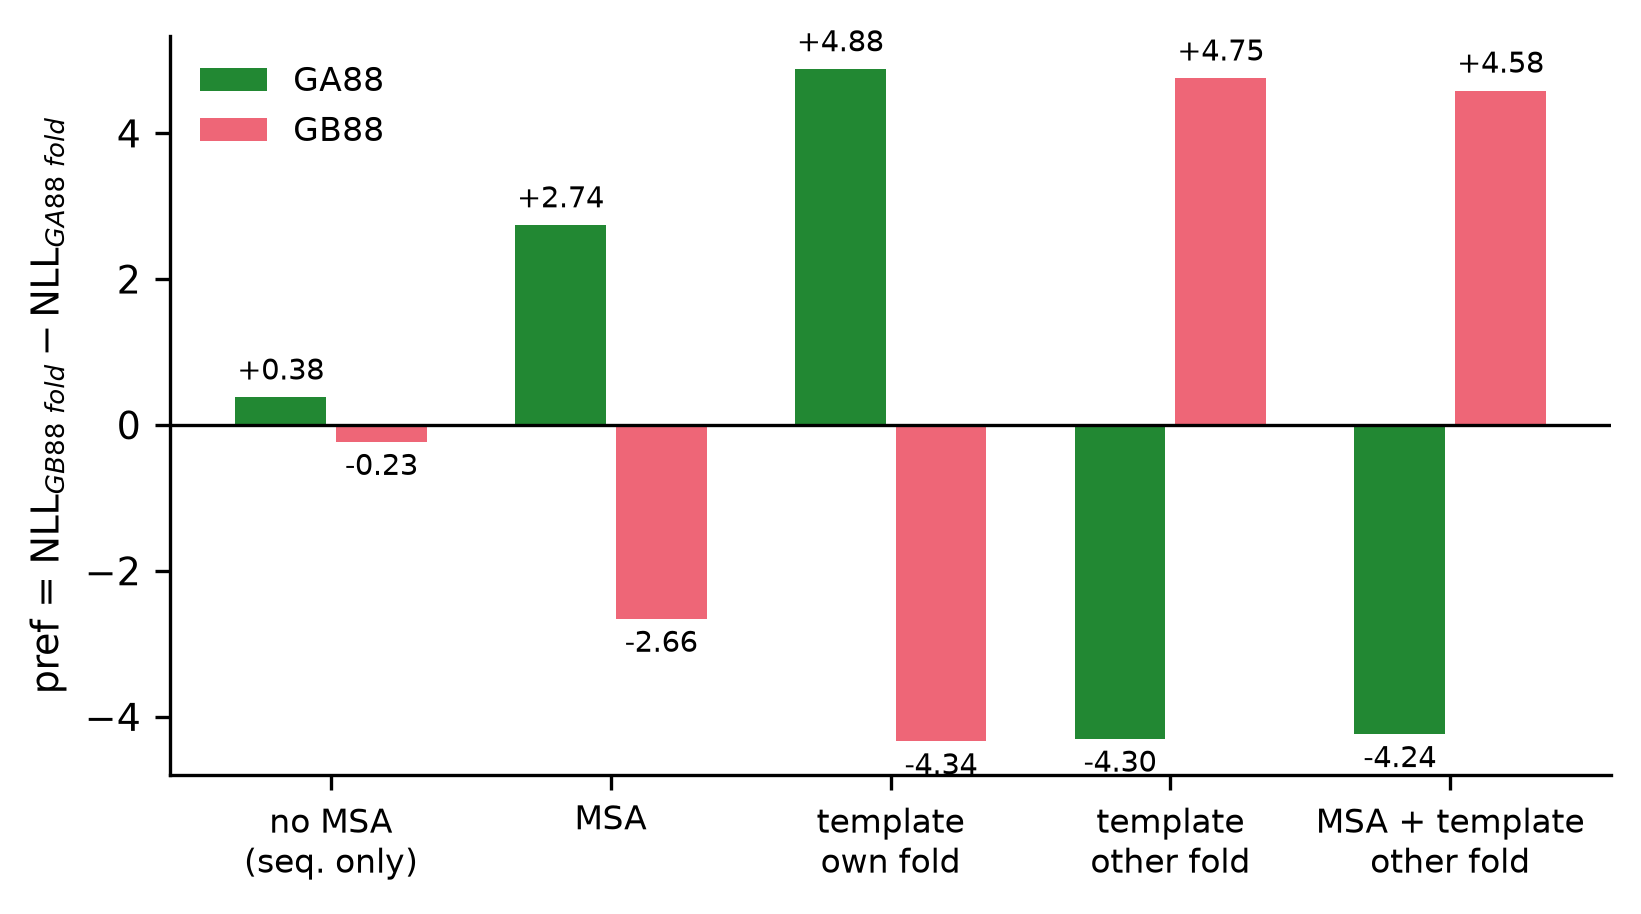
\includegraphics[width=0.9\linewidth]{figures/fig3_e49b_gagb.png}
\caption{\textbf{An opposite-fold template flips the designed GA88/GB88 pair
even against sequence and MSA.} Preference (positive favours the GA88
3$\alpha$-helix fold) for both sequences under five input conditions. All
four nomsa/msa values and both template arms are shown; the arms are nearly
mirror-symmetric between the two 88\%-identical sequences.}
\label{fig:gagb}
\end{figure}

The designed pair makes the ordering quantitative
(Fig.~\ref{fig:gagb}). Sequence alone sets only a weak own-fold preference
(GA88 $+0.38$, GB88 $-0.23$). The MSA amplifies it to $\pm 2.7$. A template
of the protein's \emph{own} fold strengthens it further ($+4.88$, $-4.34$),
and a template of the \emph{opposite} fold reverses it outright
($-4.30$, $+4.75$) --- even in combination with the sequence's own MSA
($-4.24$, $+4.58$). In RF3 the conformational state-selection hierarchy is
therefore template ($\pm 4$--$5$) $>$ MSA ($\pm 2.7$) $>$ sequence
($\pm 0.2$--$0.4$). This contrasts with AF2, where memorized folds resist
alternative templates \cite{chakravarty2024} and strong MSAs override
template information \cite{kovalevskiy2024}; we return to the likely
mechanistic reason in the Discussion.

One target requires an honest caveat. For Mad2, the state-A template (the
O-state NMR structure 1DUJ) barely pulls toward A (tplA $-0.17$ vs
sequence-only $-0.05$), while the state-B template works as expected
($-1.87$). 1DUJ is an N-terminal truncation and an NMR ensemble rather than
a crystal structure; construct mismatch or ensemble averaging plausibly
blunt its template effect. We report the anomaly rather than smoothing over
it, and note that the conflict conclusion above does not depend on this arm.

\subsection{A crystal template is not an MSA: three levels of falsification,
and opposite functional signs}

If the MSA's effect were equivalent to supplying a crystallographic
template, the two should look alike wherever we look. They do not. We
compared, on the SARS-CoV-2 spike receptor-binding domain (RBD), the pair
representations and the downstream predictability produced by the wild-type
crystal template 6M0J \cite{lan2020} versus a 15-row MSA, against the no-MSA
reference (Fig.~\ref{fig:rbd}, Table~\ref{tab:rbd}).

At the \textbf{output-preference} level (Section above), the template
dominates the MSA in conflict; the MSA does not mimic the template.
At the \textbf{representation} level, both priors compress the effective
rank of the pair representation (MSA $181 \rightarrow 139$, template $181
\rightarrow 160$), but the writes differ qualitatively: the template rotates
the representation further from the no-MSA reference (CKA $0.443$ vs
$0.568$), scrambles per-mutant delta directions harder (median cosine to the
no-MSA delta $0.26$ vs $0.48$), and amplifies mutation-delta norms more
($1.51$ vs $1.21$). The two arms themselves are only moderately similar
(CKA(template, MSA) $= 0.482$), and the combined arm is indistinguishable
from the template alone on every metric ($|\Delta| \le 0.01$) --- the
template dominates geometrically as well.
At the \textbf{functional} level, the contrast is sharpest: predicting
per-position mutation effects from the pair representation (RBD DMS,
500-mutant subset, 5 splits $\times$ 3 initializations, cross-position
Spearman $\rho$), the 15-row MSA improves over no-MSA ($0.638$ vs $0.415$,
$+0.223$ in this protocol; a de-biased full-set estimate of the MSA effect
is $+0.14$--$0.15$ \emph{in the same direction}), while the crystal template
is \emph{worse than supplying no evolutionary information at all} ($0.366$,
$-0.049$ relative to no-MSA), and adding the MSA to the template does not
rescue it ($0.370$).

\begin{figure}[t]
\centering
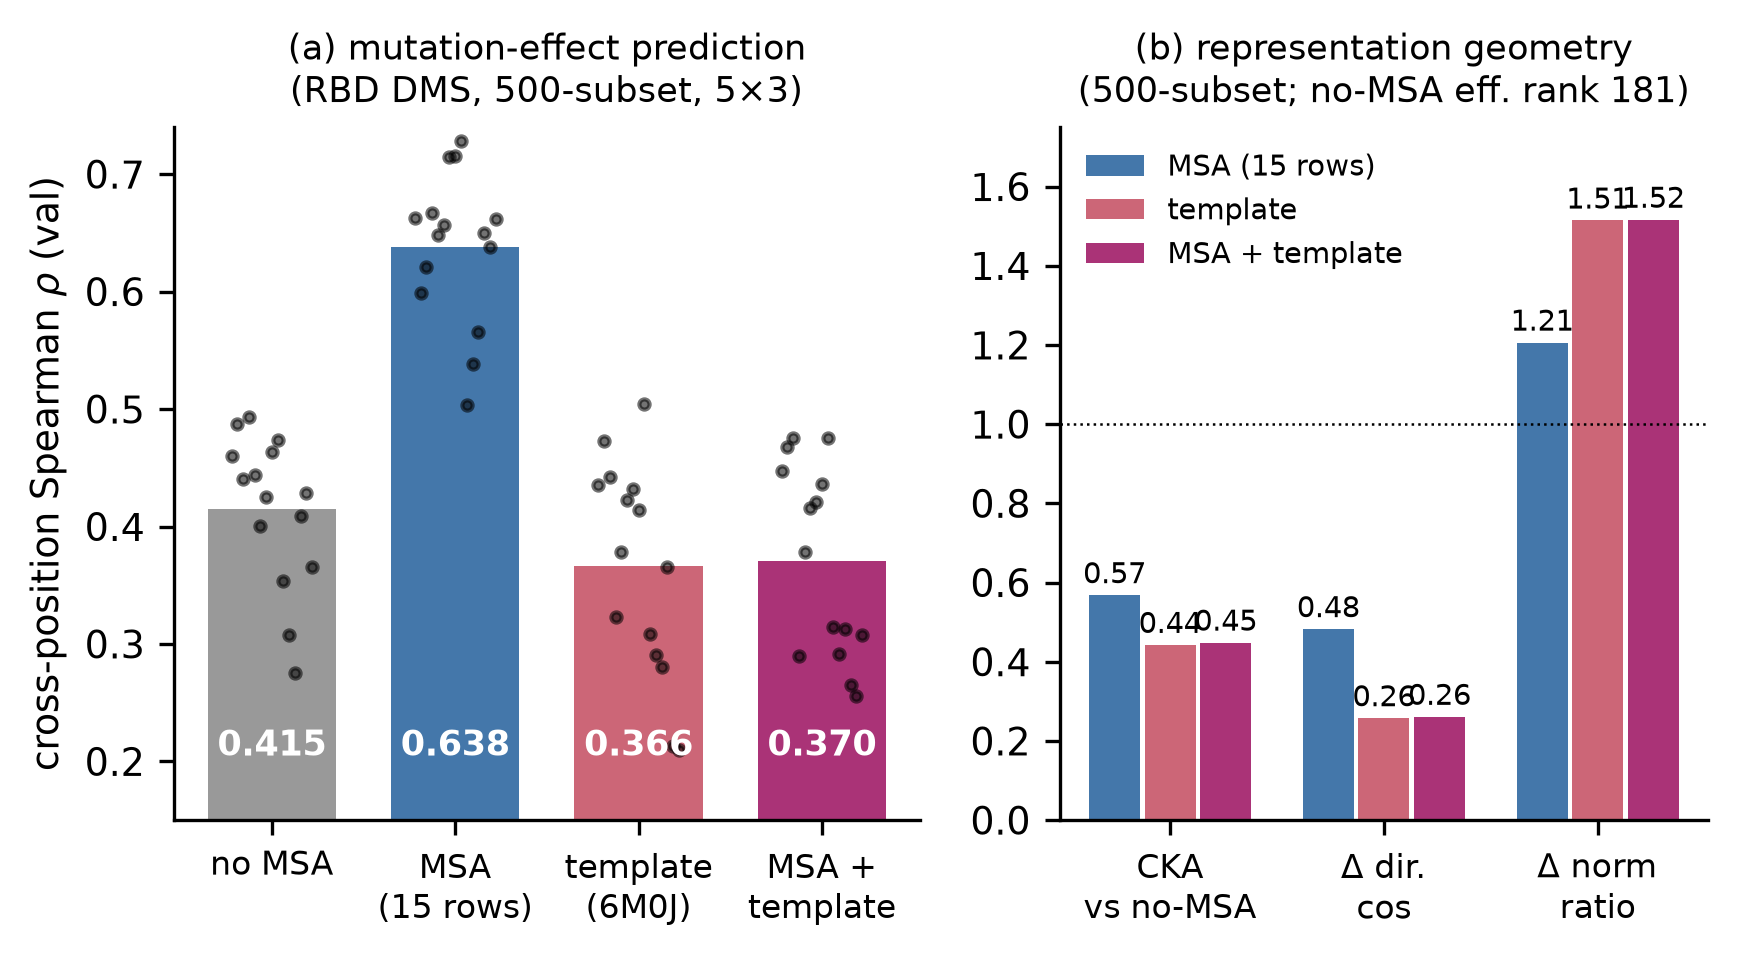
\includegraphics[width=0.98\linewidth]{figures/fig5_e49rbd.png}
\caption{\textbf{Template and MSA writes differ geometrically and diverge in
function.} (a) Cross-position Spearman correlation of predicted versus
measured mutation effects on the RBD (dots: 15 split$\times$init runs; bar:
mean). The MSA helps; the wild-type crystal template harms. (b) Pair
representation geometry relative to the no-MSA arm: CKA similarity, median
cosine of mutation-delta directions, median mutation-delta norm ratio. The
template arm is a stronger, more disruptive rewrite, and the combined arm
tracks the template.}
\label{fig:rbd}
\end{figure}

The mechanistic reading is that the template's write is mutation-erasing:
because the template track is trained on ground-truth structures, it pulls
every mutant's pair representation toward the wild-type crystal, collapsing
exactly the variation a DMS predictor needs. ``Prior strength'' and
``content type'' are independent axes: the template is the stronger prior
yet carries the wrong content for variant analysis, while the MSA's milder
write carries family-consensus content that is directly useful. Any
temptation to think of the MSA as ``a crystallographic template in
disguise'' --- a natural reading of the AF2-era state-bias literature
\cite{heo2022,sala2023} --- is falsified at all three levels in this trunk.

\subsection{Inter-chain amplification is an internal interface prior, not
paired-alignment coevolution}

Finally we asked whether the MSA's influence includes inter-chain
coevolution, using human caspase-3 (CASP3), an obligate homodimer modelled
as a 488-token two-chain input \cite{roychowdhury2022}. Across 392 mutants,
the MSA restructures the within-chain blocks of the pair representation only
moderately (median cosine between MSA and no-MSA blocks $0.712$ for A--A and
$0.712$ for B--B) while the inter-chain A--B block is both better preserved
in direction ($0.749$; A--B minus A--A $= +0.037$, paired Wilcoxon
$p = 5.5\times10^{-66}$) and markedly amplified in norm (ratio $1.28$ vs
$1.05$ within-chain). This is the signature of the network ``docking'' the
two chains more emphatically when family context is present.

To test whether this requires true inter-chain coevolution --- homolog rows
paired by species across the two chains --- we repeated the extraction with
the chain-B alignment rows shuffled to destroy row-wise pairing. The block
statistics are identical to the paired run to three decimal places
(Fig.~\ref{fig:e3}: A--A $0.713/1.055$, B--B $0.712/1.054$, A--B
$0.749/1.280$; A--B minus A--A $+0.037$, $p = 3.9\times10^{-18}$; $n = 100$
mutants), even though per-mutant embeddings differ between the two MSAs at
cosine $0.969$ (the level expected from alignment subsampling noise).
Amplifying the interface therefore does not require pairing information: the
MSA's family context switches on (or turns up) an interface prior already
present in the trunk. This is consistent with reports that paired alignments
are often unnecessary for complex prediction \cite{mirdita2022,lin2023}, and
it sharpens them: at the representation level the effect of the MSA on the
interface is not a coevolutionary docking signal at all.

\begin{figure}[t]
\centering
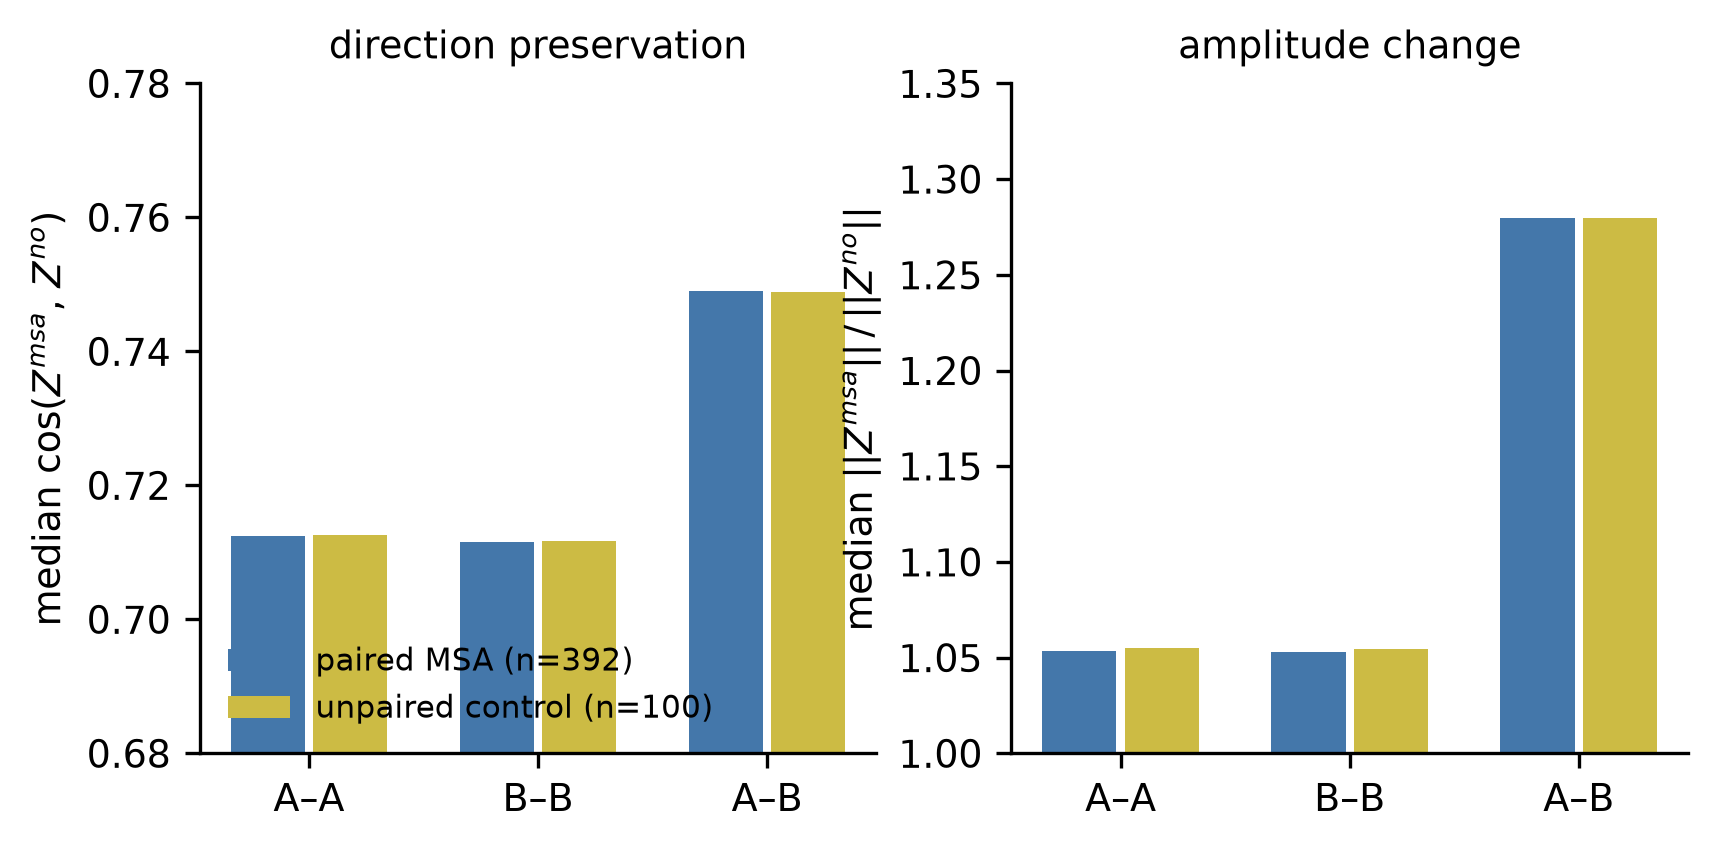
\includegraphics[width=0.98\linewidth]{figures/fig4_e3_blocks.png}
\caption{\textbf{Inter-chain amplification survives destruction of row
pairing.} Block decomposition of the MSA effect on the CASP3 homodimer pair
representation for the paired MSA (blue) and an unpaired control in which
chain-B homolog rows were shuffled (yellow). Left: direction preservation
(median cosine with the no-MSA block). Right: amplitude change (median norm
ratio). The cross-chain block is preferentially amplified in both runs,
identically.}
\label{fig:e3}
\end{figure}

\section{Discussion}

Our results support three claims, all scoped to AF3-style trunks as
implemented in RF3. First, the MSA's conformational influence is a
family-consensus state selection: its direction is set by which state the
family statistics favour, which may be the crystallized state (XCL1, Mad2),
the alternative state (KaiB, RfaH), or merely a sharpening of the
sequence-intrinsic preference (GA88/GB88), and is absent on targets whose
family is uninformative or whose states differ subtly. Second, the input
hierarchy of AF2 is inverted: a ground-truth-trained template channel
steers state preference by $\pm 4$--$5$ NLL units, dominates the MSA in
direct conflict on every target tested, and flips even a designed fold pair
against its own MSA, while the sequence alone contributes only
$\pm 0.2$--$0.4$. Third, ``the MSA as a de facto crystal template'' fails
on three independent levels, and the sign of the functional effect separates
the two channels: family-consensus content helps mutation-effect prediction,
a wild-type template hurts it.

\paragraph{Why might the hierarchy be inverted?}
The most parsimonious explanation is architectural. AF2 regularized its
template track and iterated MSA--pair exchange over 48 Evoformer blocks; its
templates were additionally downweighted by design choices such as template
dropout during training, and empirically a strong MSA overrides templates
\cite{jumper2021,kovalevskiy2024}. AF3-style models demote the MSA to a
one-shot, pair-weighted write and simultaneously train the template track
against noised ground-truth atom coordinates \cite{abramson2024,corley2025},
a regime that plausibly instils a literal-copying prior: the network has
been rewarded, during training, for reproducing supplied structure. Under
that prior, a template should behave like a near-irresistible instruction,
which is what we observe. The same mechanism explains why the template write
is mutation-erasing for DMS prediction: the copying prior has no notion of
the query differing from the template.

\paragraph{Model specificity.}
This caveat deserves emphasis. Every number in this paper comes from one
model (RF3), one checkpoint, and one inference configuration. AF2 and AF3
regularize their template channels differently, and other AF3-style
implementations may place the template--MSA balance elsewhere. We therefore
present the inverted hierarchy as a property of RF3's ground-truth-trained
template channel and a demonstration that the AF2 ordering is not a law of
the architecture family --- not as a universal claim about all
MSA-using predictors. The cleanest cross-model test would repeat the
conflict arms of Fig.~\ref{fig:e49} and Fig.~\ref{fig:gagb} in AF2 and AF3
proper.

\paragraph{Practical implications.}
For practitioners sampling alternative conformations, the AF2-era playbook
--- weaken or recluster the MSA to release alternative states
\cite{delalamo2022,stein2022,wayment2024,kalakoti2025} --- may be less
effective, and less necessary, in AF3-style models: in RF3 the state is
chosen primarily by the template track, so supplying a template of the
desired state is the direct lever, and MSA manipulation becomes the
secondary one. Conversely, users of AF3-style models for variant-effect or
stability analysis should be aware that structural templates can actively
degrade mutation-conditioned signal, while the MSA helps; and that
MSA-driven interface amplification in homomers does not by itself evidence
inter-chain coevolution.

\paragraph{Relation to the wider literature.}
Our measurements sit between two established observations. On one side, the
claim that AF2-class networks learn an MSA--structure relationship rather
than a sequence--structure relationship \cite{ahdritz2024,vargas2025} is
borne out here in a precise sense: sequence alone barely moves the state
preference ($\pm 0.2$--$0.4$), while family context moves it by up to
$\pm 3$. On the other side, the MSA-perturbation literature shows that
conformational diversity can also be released by network stochasticity
alone, without touching the MSA \cite{wallner2023}, so input channels are
not the only lever on state choice --- and, in RF3, our conflict experiments
show they are not even the strongest one. We also note a qualification our
panel adds to the fold-switching literature: AF2's reported failure on fold
switchers is partly memorization \cite{chakravarty2024}; RF3, tested on a
partly overlapping target set, gets the designed GA88/GB88 pair right from
sequence alone, so fold-switch difficulty is itself model-dependent.

\paragraph{Limitations.}
(i) Each conformational preference rests on a single forward pass per
condition; our noise band ($\pm 0.14$--$0.27$) was estimated from repeat
runs, and all headline shifts exceed it by at least $3\times$, but seed
replicates would tighten the small effects we call null. (ii) The NLL
preference is a distogram-level readout over shared residue universes, not a
structure-level RMSD classification; it is sensitive and
template-artifact-free, but it measures preference, not sampled ensembles.
(iii) The two-state framing is a simplification --- several targets
populate more than two states. (iv) The Mad2 O-state template anomaly is
unresolved; we favour a construct/ensemble explanation but cannot exclude a
deeper asymmetry in the template channel. (v) The RBD functional comparison
uses a single (if standard) DMS dataset and a shallow 15-row MSA; the sign
contrast is the claim, not the exact effect sizes. (vi) Our conclusions draw
on a corrected analysis pipeline: a first-pass scoring bug (states scored on
non-shared residue spans, plus a 14-residue misalignment from a compressed
disordered loop in the RfaH reference) inflated some shifts and manufactured
others (LacY, EGFR), and an early template run silently dropped the template
input; we report only post-correction values and regard the discarded
analyses as cautionary, not evidentiary.

\section{Methods}

\subsection{Model and inference}
All experiments use RosettaFold-3 \cite{corley2025}, an open implementation
of the AF3 architecture, with a single checkpoint and inference settings
held fixed throughout: 10 recycles, diffusion sampling with 50 steps and
diffusion batch size 2. Per condition we record the distogram head logits
(64 distance bins over 2--22\,\AA\ plus a no-contact bin) and the final pair
representation. Template inputs are supplied through RF3's token-level
template track; template tokens are appended after query tokens in the
modelled assembly, and query regions are sliced by component length for
scoring.

\subsection{Targets, structures, and MSAs}
Thirteen two-state targets (Table~\ref{tab:targets}) were curated from the
fold-switching and conformational-diversity literature, with PDB accessions,
constructs and chain choices verified against RCSB and PDBe SIFTS mappings.
MSAs were built against UniRef30 (query plus up to 256 homologous rows;
actual depths in Table~\ref{tab:targets}). Templates for the conflict
experiments were single-chain mmCIFs filtered from the corresponding state
structures (chains kept under their original identifiers to avoid a silent
template-dropping failure of the input pipeline; each template input was
verified to produce a nonzero templated-atom count before inference). For
GA88/GB88 the two state structures are the NMR models 2JWS and 2JWU
\cite{alexander2007}; the RBD template is the RBD chain of 6M0J
\cite{lan2020}.

\subsection{Conformational-state preference score}
For each target and condition, we compute the mean negative log-likelihood
of the experimental C$\alpha$--C$\alpha$ distances of each state under the
predicted distogram:
$\mathrm{NLL}_S = -\frac{1}{|\mathcal{P}|}\sum_{(i,j)\in\mathcal{P}}
\log p_{ij}(d^{S}_{ij})$,
where $S \in \{A,B\}$ and $\mathcal{P}$ is the pair set. The state
preference is $\pref = \mathrm{NLL}_B - \mathrm{NLL}_A$ (positive favours
state A). \textbf{Range matching:} each state's experimental map is aligned
to the folded query sequence by sequence alignment (minimum matching block
5 residues), and $\mathcal{P}$ is restricted to residue pairs that are
covered by \emph{both} states' maps and finite in both, so that every
preference compares identical residue pairs on both sides. This corrects
the first-pass analysis, in which states were scored on their own spans
(creating artificial preferences, e.g.\ LacY, EGFR) and a compressed
disordered loop (UniProt 101--114 missing in the RfaH state-A reference)
misaligned rows by 14 residues; all pre-correction magnitudes are superseded
by the values reported here. The run-to-run noise band of $\pref$ shifts
($\pm 0.14$--$0.27$) was estimated from archived repeat forwards of
identical inputs. Steering and conflict measures are
$\mathrm{steer}_{\mathrm{tpl}} = \pref_{\mathrm{tplB}} -
\pref_{\mathrm{tplA}}$ and $\mathrm{conflict} = \pref_{\mathrm{msa,tplA}} -
\pref_{\mathrm{tplA}}$.

\subsection{Representation geometry and supervised evaluation on RBD}
Pair representations were extracted for a 500-mutant subset of the
SARS-CoV-2 RBD DMS dataset \cite{starr2020} under four input conditions:
no-MSA, a 15-row MSA, the 6M0J RBD template, and MSA-plus-template.
Geometry metrics per arm: effective rank (number of singular values needed
for 90\% of variance), linear CKA against the no-MSA arm, and per-mutant
delta statistics (median cosine and median norm ratio of the mutant-minus-WT
representation change relative to the no-MSA arm). Supervised evaluation
trained a mutation-effect predictor on frozen representations with
per-position standardization, using 5 cross-position splits (30\% of
positions held out) $\times$ 3 initializations, and reports best-epoch
validation Spearman correlation; the de-biased full-set MSA effect quoted in
the text ($+0.14$--$0.15$) comes from held-out-test and strict
(train-only) standardization variants of the same pipeline on the full
3{,}998-mutant set.

\subsection{Homodimer block analysis and the unpaired control}
CASP3 was modelled as a two-chain, 488-token homodimer. For each of 392
mutants (stride-4 subset of the DMS set) we computed, per block
(A--A, B--B, A--B) of the full pair representation, the cosine similarity
and norm ratio between the MSA and no-MSA extractions, plus a paired
Wilcoxon signed-rank test of A--B versus A--A cosines. The unpaired control
re-ran the extraction with the chain-B MSA rows shuffled to destroy
species-level pairing (100 mutants), using the same pipeline and statistics.

\subsection{Reproducibility}
Analysis scripts, target definitions, and all reported numbers are archived
with the project; every figure is generated directly from archived JSON
result files (\texttt{make\_figs.py}). A claim-by-claim traceability table
(\texttt{TRACEABILITY.md}) maps each quantitative statement to its source
file.

\section*{Data availability}
All structures used are public (PDB IDs in Table~\ref{tab:targets}). DMS
data are from published datasets \cite{starr2020,roychowdhury2022}. RF3 is
publicly available \cite{corley2025}. Analysis code, inputs, and archived
result files are publicly available at
\url{https://github.com/Lizon1c/rf3-state-selection}.

\section*{Acknowledgements}
The author thanks the developers of RoseTTAFold3 for an open implementation
of the AlphaFold3-style architecture. No external funding was received for
this work.

\section*{Funding}
No external funding was received for this work.

\section*{Competing interests}
The author declares no competing interests.

\begin{thebibliography}{99}

\bibitem{jumper2021}
Jumper J, et al. Highly accurate protein structure prediction with
AlphaFold. \emph{Nature} 596:583--589 (2021).

\bibitem{abramson2024}
Abramson J, et al. Accurate structure prediction of biomolecular
interactions with AlphaFold 3. \emph{Nature} 630:493--500 (2024).

\bibitem{corley2025}
Corley M, et al. AtomWorks and RosettaFold-3. \emph{bioRxiv}
2025.08.14.670328 (2025).

\bibitem{kovalevskiy2024}
Kovalevskiy O, Mateos-Garcia J, Tunyasuvunakool K. AlphaFold two years on:
validation and impact. \emph{Proc.\ Natl.\ Acad.\ Sci.\ USA}
121(34):e2315002121 (2024).

\bibitem{lin2023}
Lin Z, et al. Evolutionary-scale prediction of atomic-level protein
structure with a language model. \emph{Science} 379:1123--1130 (2023).

\bibitem{hayes2024}
Hayes T, et al. Simulating 500 million years of evolution with a language
model. \emph{Science} 385:eado9336 (2024); preprint:
bioRxiv 2024.07.01.600583.

\bibitem{watson2023}
Watson JL, et al. De novo design of protein structure and function with
RFdiffusion. \emph{Nature} 620:1075--1084 (2023).

\bibitem{senior2020}
Senior AW, et al. Improved protein structure prediction using potentials
from deep learning. \emph{Nature} 577:706--710 (2020).

\bibitem{marks2012}
Marks DS, Hopf TA, Sander C. Protein structure prediction from sequence
variation. \emph{Nat.\ Struct.\ Mol.\ Biol.} 19:1293--1301 (2012).

\bibitem{delalamo2022}
del Alamo D, Sala D, Mchaourab HS, Meiler J. Sampling alternative
conformational states of transporters and receptors with AlphaFold2.
\emph{eLife} 11:e75751 (2022).

\bibitem{stein2022}
Stein RA, Mchaourab HS. SPEACH\_AF: sampling protein ensembles and
conformational heterogeneity with AlphaFold2. \emph{PLoS Comput.\ Biol.}
18(8):e1010483 (2022).

\bibitem{wayment2024}
Wayment-Steele HK, et al. Predicting multiple conformations via sequence
clustering and AlphaFold2. \emph{Nature} 625:832--839 (2024).

\bibitem{kalakoti2025}
Kalakoti Y, Wallner B. AFsample2 predicts multiple conformations and
ensembles with AlphaFold2. \emph{Commun.\ Biol.} 8:373 (2025).

\bibitem{wallner2023}
Wallner B. AFsample: improving multimer prediction with AlphaFold using
massive sampling. \emph{Bioinformatics} 39(9):btad573 (2023).

\bibitem{chakravarty2024}
Chakravarty D, et al. AlphaFold predictions of fold-switched conformations
are driven by structure memorization. \emph{Nat.\ Commun.} 15:7296 (2024).

\bibitem{chakravarty2022}
Chakravarty D, Porter LL. AlphaFold2 fails to predict protein fold
switching. \emph{Protein Sci.} 31(6):e4353 (2022).

\bibitem{saldano2022}
Salda\~no TE, et al. Impact of protein conformational diversity on
AlphaFold predictions. \emph{Bioinformatics} 38(10):2742--2748 (2022).

\bibitem{sala2023}
Sala D, Hildebrand PW, Meiler J. Biasing AlphaFold2 to predict GPCRs and
kinases with user-defined functional or structural properties.
\emph{Front.\ Mol.\ Biosci.} 10:1121962 (2023).

\bibitem{heo2022}
Heo L, Feig M. Multi-state modeling of G-protein coupled receptors at
experimental accuracy. \emph{Proteins} 90(11):1873--1885 (2022).

\bibitem{mirdita2022}
Mirdita M, et al. ColabFold: making protein folding accessible to all.
\emph{Nat.\ Methods} 19:679--682 (2022).

\bibitem{notin2023}
Notin P, et al. ProteinGym: large-scale benchmarks for protein fitness
prediction and design. \emph{NeurIPS 2023 Datasets and Benchmarks}
36:64331--64379 (2023).

\bibitem{akiyama2025}
Akiyama Y, Zhang Z, Mirdita M, Steinegger M, Ovchinnikov S. Scaling down
protein language modeling with MSA Pairformer. \emph{bioRxiv}
2025.08.02.668173 (2025).

\bibitem{vargas2025}
Vargas-Rosales E, Caflisch A. The physics--AI dialogue in drug design.
\emph{RSC Med.\ Chem.} (2025). doi:10.1039/d4md00869c.

\bibitem{ahdritz2024}
Ahdritz G, et al. OpenFold: retraining AlphaFold2 yields new insights into
its learning mechanisms and capacity for generalization. \emph{Nat.\
Methods} 21:1514--1524 (2024).

\bibitem{porter2018}
Porter LL, Looger LL. Extant fold-switching proteins are widespread.
\emph{Proc.\ Natl.\ Acad.\ Sci.\ USA} 115(23):5968--5973 (2018).

\bibitem{alexander2007}
Alexander PA, He Y, Chen Y, Orban J, Bryan PN. The design and
characterization of two proteins with 88\% sequence identity but different
structure and function. \emph{Proc.\ Natl.\ Acad.\ Sci.\ USA}
104(29):11963--11968 (2007).

\bibitem{chang2015}
Chang YG, et al. A protein fold switch joins the circadian oscillator to
clock output in cyanobacteria. \emph{Science} 349:324--328 (2015).

\bibitem{burmann2012}
Burmann BM, et al. An $\alpha$-helix to $\beta$-barrel domain switch
transforms the transcription factor RfaH into a translation factor.
\emph{Cell} 150(2):291--303 (2012).

\bibitem{luo2004}
Luo X, Tang Z, Xia G, Wassmann K, Matsumoto T, Rizo J, Yu H. The Mad2
spindle checkpoint protein has two distinct natively folded states.
\emph{Nat.\ Struct.\ Mol.\ Biol.} 11:338--345 (2004).

\bibitem{tuinstra2008}
Tuinstra RL, et al. Interconversion between two unrelated protein folds in
the lymphotactin native state. \emph{Proc.\ Natl.\ Acad.\ Sci.\ USA}
105:5057--5062 (2008).

\bibitem{starr2020}
Starr TN, et al. Deep mutational scanning of SARS-CoV-2 receptor binding
domain reveals constraints on folding and ACE2 binding. \emph{Cell}
182(5):1295--1310.e20 (2020).

\bibitem{roychowdhury2022}
Roychowdhury H, Romero PA. Microfluidic deep mutational scanning of the
human executioner caspases reveals differences in structure and regulation.
\emph{Cell Death Discov.} 8 (2022). doi:10.1038/s41420-021-00799-0.

\bibitem{lan2020}
Lan J, et al. Structure of the SARS-CoV-2 spike receptor-binding domain
bound to the ACE2 receptor. \emph{Nature} 581:215--220 (2020).

\end{thebibliography}

\clearpage

% ============================================================ TABLES
\begin{table}[t]
\centering
\caption{\textbf{Thirteen two-state targets and range-matched MSA-induced
shifts.} $\pref = \mathrm{NLL}_B - \mathrm{NLL}_A$ (positive favours state
A); shift $= \pref_{\mathrm{msa}} - \pref_{\mathrm{nomsa}}$. Direction is
relative to the crystallized (PDB-dominant) state. MSA rows include the
query. Noise band of the shift: $\pm 0.14$--$0.27$. XR = X-ray.}
\label{tab:targets}
\scriptsize
\setlength{\tabcolsep}{3.5pt}
\begin{tabular}{llllrrrrrl}
\toprule
Target & Category & State A (PDB) & State B (PDB) & MSA rows & res. &
$\pref_{\mathrm{no}}$ & $\pref_{\mathrm{msa}}$ & shift & direction \\
\midrule
KaiB & fold-sw. & 2QKE XR GS & 5JYT NMR FS & 257 & 90 & $+0.72$ & $-1.57$ & $-2.29$ & away \\
RfaH & fold-sw. & 2OUG XR $\alpha$ & 2LCL NMR $\beta$ & 257 & 42 & $+0.10$ & $-2.89$ & $-2.99$ & away \\
Mad2 & fold-sw. & 1DUJ NMR O & 1S2H NMR C$^{\dagger}$ & 257 & 184 & $-0.05$ & $-0.96$ & $-0.91$ & toward \\
XCL1 & fold-sw. & 1J8I NMR chemok. & 2JP1 NMR $\beta$-sand. & 160 & 39 & $-0.78$ & $+2.09$ & $+2.87$ & toward \\
selecase & fold-sw. & 4QHF XR mon. & 4QHJ XR olig. & 2 & 105 & $+0.13$ & $+0.13$ & $-0.01$ & null \\
GA88/GB88 & designed & 2JWS NMR 3$\alpha$ & 2JWU NMR $\alpha/\beta$ & 24 & 40 & $+0.52$ & $+3.07$ & $+2.56$ & sharpen$^{\ddagger}$ \\
$\beta$2AR & GPCR & 2RH1 XR inact. & 3SN6 XR act. & 257 & 271 & $-0.06$ & $+0.09$ & $+0.15$ & null \\
Abl1 & kinase & 2GQG XR DFG-in & 2HYY XR DFG-out & 257 & 262 & $-0.00$ & $+0.01$ & $+0.01$ & null \\
EGFR & kinase & 1M17 XR $\alpha$C-in & 1XKK XR $\alpha$C-out & 257 & 265 & $+0.14$ & $+0.12$ & $-0.02$ & null \\
LacY & transporter & 1PV6 XR inward & 4OAA XR outward & 257 & 388 & $+0.06$ & $-0.01$ & $-0.08$ & null \\
ubiquitin & XR/NMR & 1UBQ XR & 1D3Z NMR & 257 & 76 & $-0.08$ & $-0.10$ & $-0.03$ & null \\
GB1 & XR/NMR & 1PGB XR & 2GB1 NMR & 89 & 55 & $+0.36$ & $+0.44$ & $+0.09$ & null \\
thioredoxin & XR/NMR & 2TRX XR ox. & 1XOA NMR ox. & 257 & 108 & $+0.26$ & $+0.38$ & $+0.13$ & null \\
\bottomrule
\end{tabular}
\begin{flushleft}\footnotesize
$^{\dagger}$For Mad2 the crystallized (PDB-dominant) state is state~B
(C-Mad2), so a negative shift points toward crystal.
$^{\ddagger}$GA88/GB88 has no single crystallized state; the shift sharpens
each sequence's own-fold preference (main-flow GA88 scoring shown; per-sequence
values in Fig.~\ref{fig:gagb}).
\end{flushleft}
\end{table}

\begin{table}[t]
\centering
\caption{\textbf{Template versus MSA steering on five two-state targets
(range-matched).} Preferences as in Table~\ref{tab:targets};
steer $= \pref_{\mathrm{tplB}} - \pref_{\mathrm{tplA}}$;
conflict $= \pref_{\mathrm{msa,tplA}} - \pref_{\mathrm{tplA}}$.
$|$conflict$| \le 0.23$ on all five: the template wins every direct
conflict with the MSA.}
\label{tab:e49}
\small
\begin{tabular}{lrrrrrrr}
\toprule
Target & $\pref_{\mathrm{no}}$ & $\pref_{\mathrm{msa}}$ &
$\pref_{\mathrm{tplA}}$ & $\pref_{\mathrm{tplB}}$ &
$\pref_{\mathrm{msa,tplA}}$ & steer & conflict \\
\midrule
KaiB & $+0.72$ & $-1.57$ & $+3.59$ & $-3.00$ & $+3.36$ & $-6.59$ & $-0.23$ \\
RfaH & $+0.10$ & $-2.89$ & $+1.49$ & $+0.30$ & $+1.45$ & $-1.19$ & $-0.04$ \\
Mad2 & $-0.05$ & $-0.96$ & $-0.17^{\dagger}$ & $-1.87$ & $-0.17$ & $-1.70$ & $+0.00$ \\
XCL1 & $-0.78$ & $+2.09$ & $-1.49$ & $-0.86$ & $-1.44$ & $+0.63$ & $+0.05$ \\
LacY & $+0.06$ & $-0.01$ & $+0.54$ & $+0.08$ & $+0.51$ & $-0.47$ & $-0.03$ \\
\bottomrule
\end{tabular}
\begin{flushleft}\footnotesize
$^{\dagger}$Mad2 anomaly: the O-state template (1DUJ, NMR ensemble,
N-terminal truncation) does not pull toward state A; see text.
\end{flushleft}
\end{table}

\begin{table}[t]
\centering
\caption{\textbf{Template versus MSA on the RBD: geometry and function}
(500-mutant subset). eff90: effective rank (90\% variance). CKA: linear CKA
vs the no-MSA arm. $\Delta$dir./norm: median cosine and norm ratio of
mutation-conditioned representation changes relative to no-MSA. Spearman:
cross-position mutation-effect prediction (mean of 5 splits $\times$ 3
inits).}
\label{tab:rbd}
\small
\begin{tabular}{lccccc}
\toprule
Arm & eff90 & CKA vs no-MSA & $\Delta$ direction & $\Delta$ norm ratio & Spearman $\rho$ \\
\midrule
no MSA & 181 & (1.00) & (1.00) & (1.00) & 0.415 \\
MSA (15 rows) & 139 & 0.568 & 0.48 & 1.21 & 0.638 \\
template (6M0J) & 160 & 0.443 & 0.26 & 1.51 & 0.366 \\
MSA + template & 159 & 0.448 & 0.26 & 1.52 & 0.370 \\
\bottomrule
\end{tabular}
\begin{flushleft}\footnotesize
CKA(template, MSA) $= 0.482$. The de-biased full-set MSA effect under the
canonical protocol is $+0.14$--$0.15$ (Methods); the $+0.223$ here reflects
the 500-subset protocol used for all four arms.
\end{flushleft}
\end{table}

\end{document}
